% BAC 2024 D - Exercice 4
% Plan complexe - Points A, B, C, I

\documentclass[border=5pt]{standalone}
\usepackage{tikz}
\usepackage{amsmath}
\usepackage{amssymb}

\begin{document}

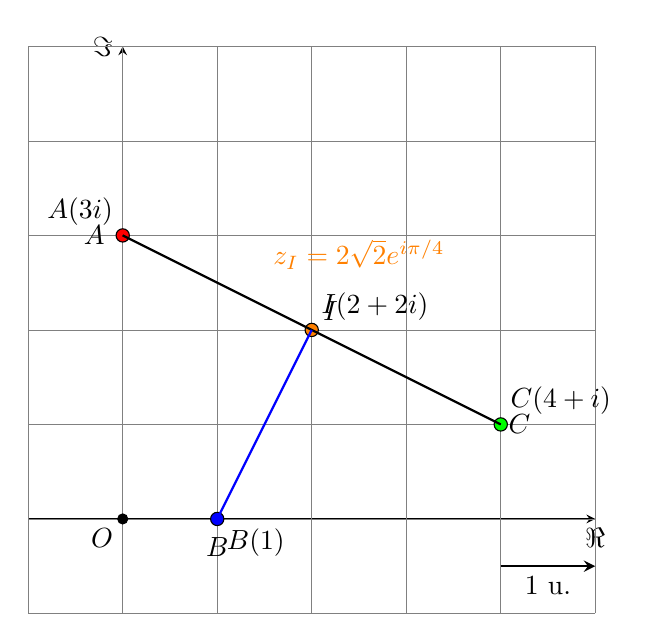
\begin{tikzpicture}[scale=1.2, >=stealth]

% Axes
\draw[->] (-1,0) -- (5,0) node[below] {$\Re$};
\draw[->] (0,-1) -- (0,5) node[left] {$\Im$};

% Grid
\draw[help lines] (-1,-1) grid (5,5);

% Point A: z_A = 3i
\coordinate (A) at (0,3);
\draw[fill=red] (A) circle (2pt) node[above left] {$A(3i)$};

% Point B: z_B = 1
\coordinate (B) at (1,0);
\draw[fill=blue] (B) circle (2pt) node[below right] {$B(1)$};

% Point C: z_C = 4 + i
\coordinate (C) at (4,1);
\draw[fill=green] (C) circle (2pt) node[above right] {$C(4+i)$};

% Point I: milieu de [AC]
\coordinate (I) at (2,2);
\draw[fill=orange] (I) circle (2pt) node[above right] {$I(2+2i)$};

% Draw segments
\draw[thick] (A) -- (C);
\draw[thick, blue] (B) -- (I);
\draw[dashed] (A) -- (I) -- (C);

% Labels
\node at (-0.3,3) {$A$};
\node at (1,-0.3) {$B$};
\node at (4.2,1) {$C$};
\node at (2.2,2.2) {$I$};

% Origin
\draw[fill=black] (0,0) circle (1.5pt) node[below left] {$O$};

% Scale
\draw[->, thick] (4,-0.5) -- (5,-0.5) node[midway, below] {1 u.};

% z_I in polar form: 2√2 e^(iπ/4) = 2√2(cos(π/4) + i sin(π/4))
\node[orange] at (2.5,2.8) {$z_I = 2\sqrt{2}e^{i\pi/4}$};

\end{tikzpicture}

\end{document}